\chapter{Working with TextInput components}

\section{Reading: Common props of TextInput component}
\subsection{placeholder}
\begin{itemize}
    \item The placeholder string displayed before the user enters anything into the text input box.
    \item Syntax:
    \begin{lstlisting}[language=Java, numbers=none]
        <TextInput 
            style={styles.input} 
            value={firstName} 
            onChangeText={onChangeFirstName} 
            placeholder={'First Name'} 
        /> 
    \end{lstlisting}
\end{itemize}

\subsection{multiline}
\begin{itemize}
    \item Boolean. When set to true, the text input can be muliple lines.
    \item By default, it is set to false, all the text that cannot fit within a single line is truncated and not visible to user.
    \item Syntax:
    \begin{lstlisting}[language=Java, numbers=none]
        <TextInput 
            style={styles.messageInput} 
            value={message} 
            onChangeText={onChangeMessage} 
            placeholder={'Please leave feedback'} 
            multiline={true} 
        />
    \end{lstlisting}
\end{itemize}

\subsection{maxLength}
\begin{itemize}
    \item This props limits the maximum number of characters that can be entered.
    \item This props accepts a number as the value.
    \item Syntax:
    \begin{lstlisting}[language=Java, numbers=none]
        <TextInput 
            style={styles.messageInput} 
            value={message} 
            onChangeText={onChangeMessage} 
            placeholder={'Please leave feedback'} 
            multiline={true} 
            maxLength={250}
        />
    \end{lstlisting}
\end{itemize}

\subsection{keyboardType}
\begin{itemize}
    \item React Native's support keyboard.
    \item number-pad, decimal-pad, numeric, email-address, phone-pad, url, ...
    \item Syntax:
    \begin{lstlisting}[language=Java, numbers=none]
        <TextInput 
            style={styles.input} 
            value={phoneNumber} 
            onChangeText={onChangePhoneNumber} 
            placeholder={'Phone Number'} 
            keyboardType={'phone-pad'} 
        />
    \end{lstlisting} 
\end{itemize}

\section{Video: Passing props to TextInput Component}
\begin{itemize}
    \item Use \texttt{secureTextEntry={true}} to hide the input text from user (Use for password).
    \item \textbf{Practice Question:} You would like to create a text input box in your app for users to enter their password. To make this more secure, you would like for the characters entered in the box to be hidden and for the box to have a limit of 14 characters. Which \texttt{TextInput} props would you pass in to accomplish this? Choose all that apply.   
    $\rightarrow$ secureTextEntry, maxLength
\end{itemize}

\begin{figure}[H]
    \centering
    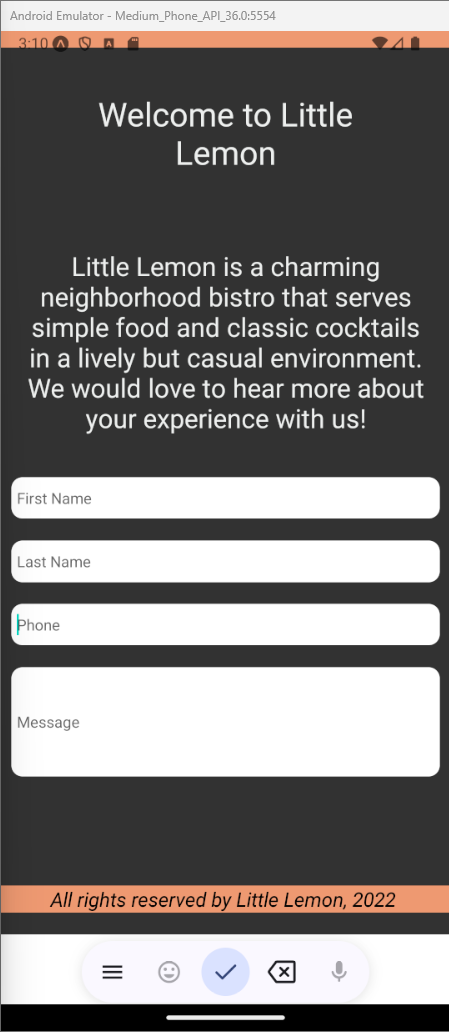
\includegraphics[width=0.2\textwidth]{images/passing-props.png}
    \caption{Passing props to TextInput Component}
\end{figure}

\section{Reading: Exercise: Create a login page}
\begin{figure}[H]
    \centering
    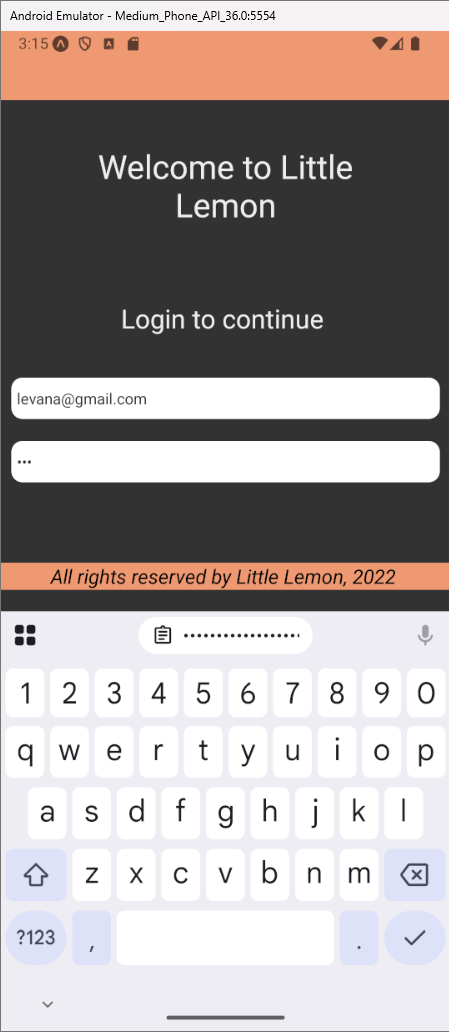
\includegraphics[width=0.2\textwidth]{images/Ex5.png}
    \caption{Exercise: Create a login page}
\end{figure}

\section{Practice Assignment: Self review: Create a login page}
\begin{figure}[H]
    \centering
    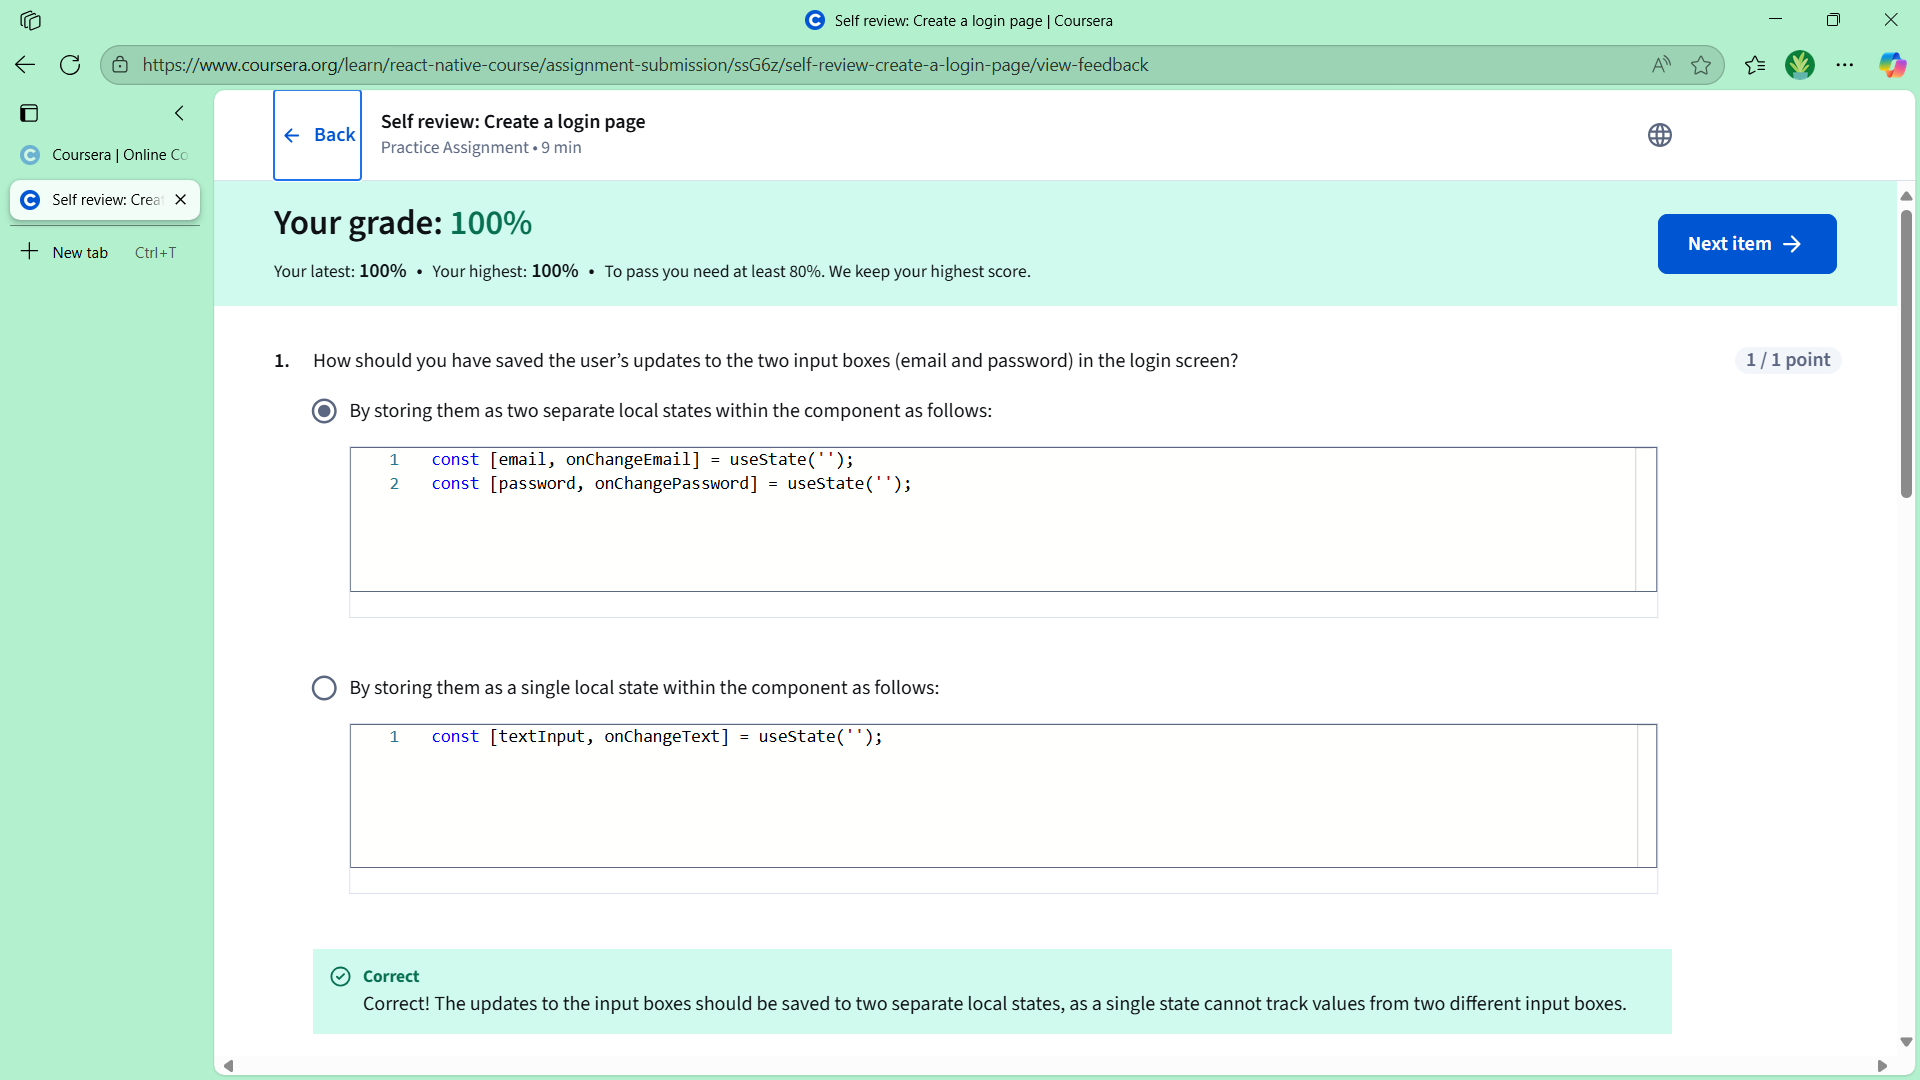
\includegraphics[width=0.5\textwidth]{images/sr-4.png}
    \caption{Self review: Create a login page}
\end{figure}

\section{Video: Using TextInput Methods}
\subsection{onFocus}
\begin{itemize}
    \item This is a callback medthod that is called when the text input is focused.
    \item $onFocus(() => \{ \})$
\end{itemize}

\subsection{onBlur}
\begin{itemize}
    \item This is also a callback method, called when the text input it remove from being focused.
    \item $onBlur(() => \{ \})$
\end{itemize}

\section{clearButtonMode}
\begin{itemize}
    \item A clear button will appear on the right side of the text box.
    \item This button allow to clear all the input text.
    \item Only support for iOS.
    \item Dont work if we have \texttt{multiline} props.
    \item clearButtonMode='always'. The default is 'never'
    \item \textbf{Practice Question:} You are creating a form for your app and would like it to display an alert whenever a user exits a certain text input box. Which prop of the \texttt{TextInput} component would you use to achieve this? 
    $\rightarrow$ onBlur
\end{itemize}

\section{Reading: TextInput Methods}
This part is the same content with above part which I have taken note clearly.

\section{Practice Assignment: Knowledge Check: Props and methods in TextInput}
\begin{figure}[H]
    \centering
    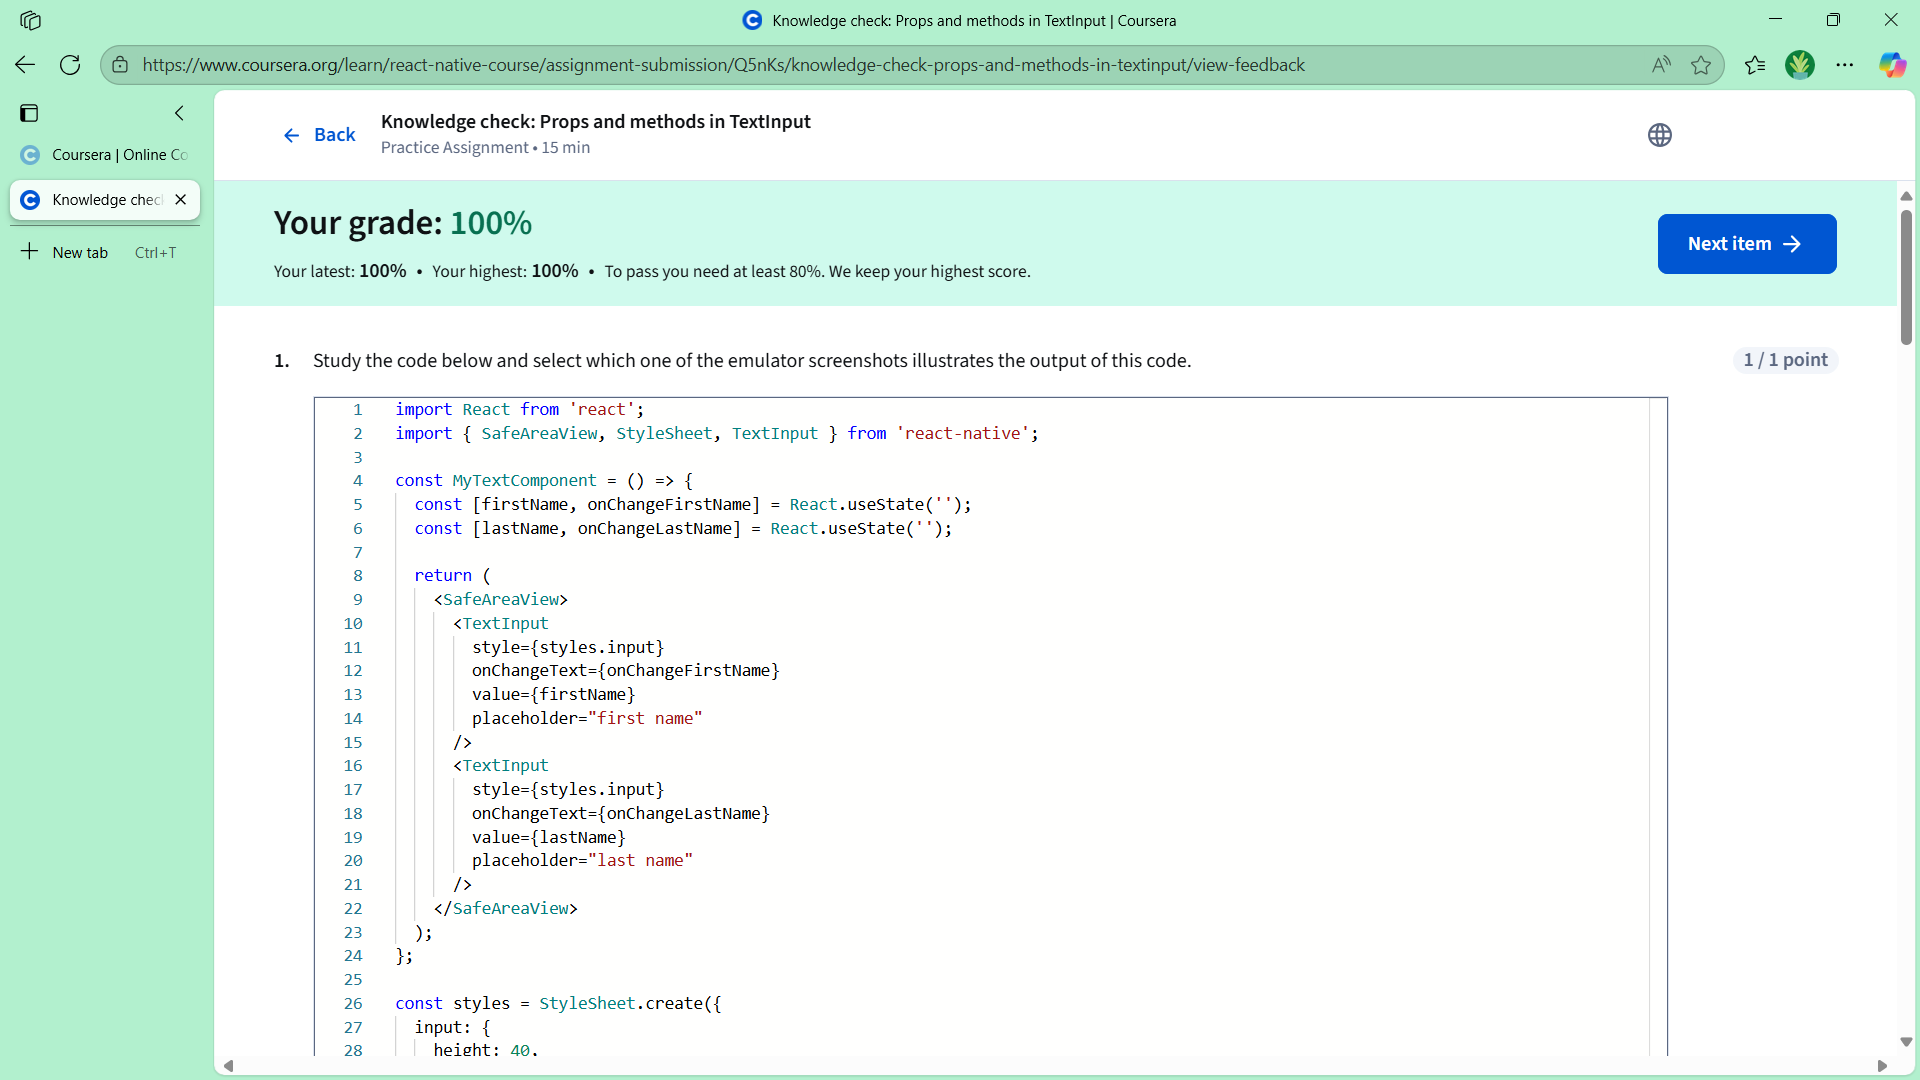
\includegraphics[width=0.5\textwidth]{images/kc-4.png}
    \caption{Knowledge Check: Props and methods in TextInput}
\end{figure}

\section{Video: Module summary: Lists and Text Input in React Native}
\begin{itemize}
    \item FlatList component
    \begin{itemize}
        \item Lazy rendering
        \item FlatList syntax
        \item Render large lists
    \end{itemize}

    \item FlatList methods
    \begin{itemize}
        \item keyExtractor
        \item ItemSeperatorComponent
        \item ListHeaderComponent
        \item ListFooterComponent
    \end{itemize}

    \item SectionList component
    \begin{itemize}
        \item Differences from FlatList
        \item SectionList syntax
        \item Render large list with sections
    \end{itemize}

    \item TextInput component
    \begin{itemize}
        \item Create text input boxes
        \item Configure TextInput
        \item Create TextInput components in ScrollView
    \end{itemize}

    \item Keyboard Handling
    \begin{itemize}
        \item keyboardDismissMode
        \item KeyboardAvoidingView
    \end{itemize}

    \item TextInput props
    \begin{itemize}
        \item Enable additional TextInput functionalities
        \item Set responses to actions in text box
    \end{itemize}
\end{itemize}

\section{Graded Assignment: Module quiz: Lists and Text Input in React Native}
\begin{figure}[H]
    \centering
    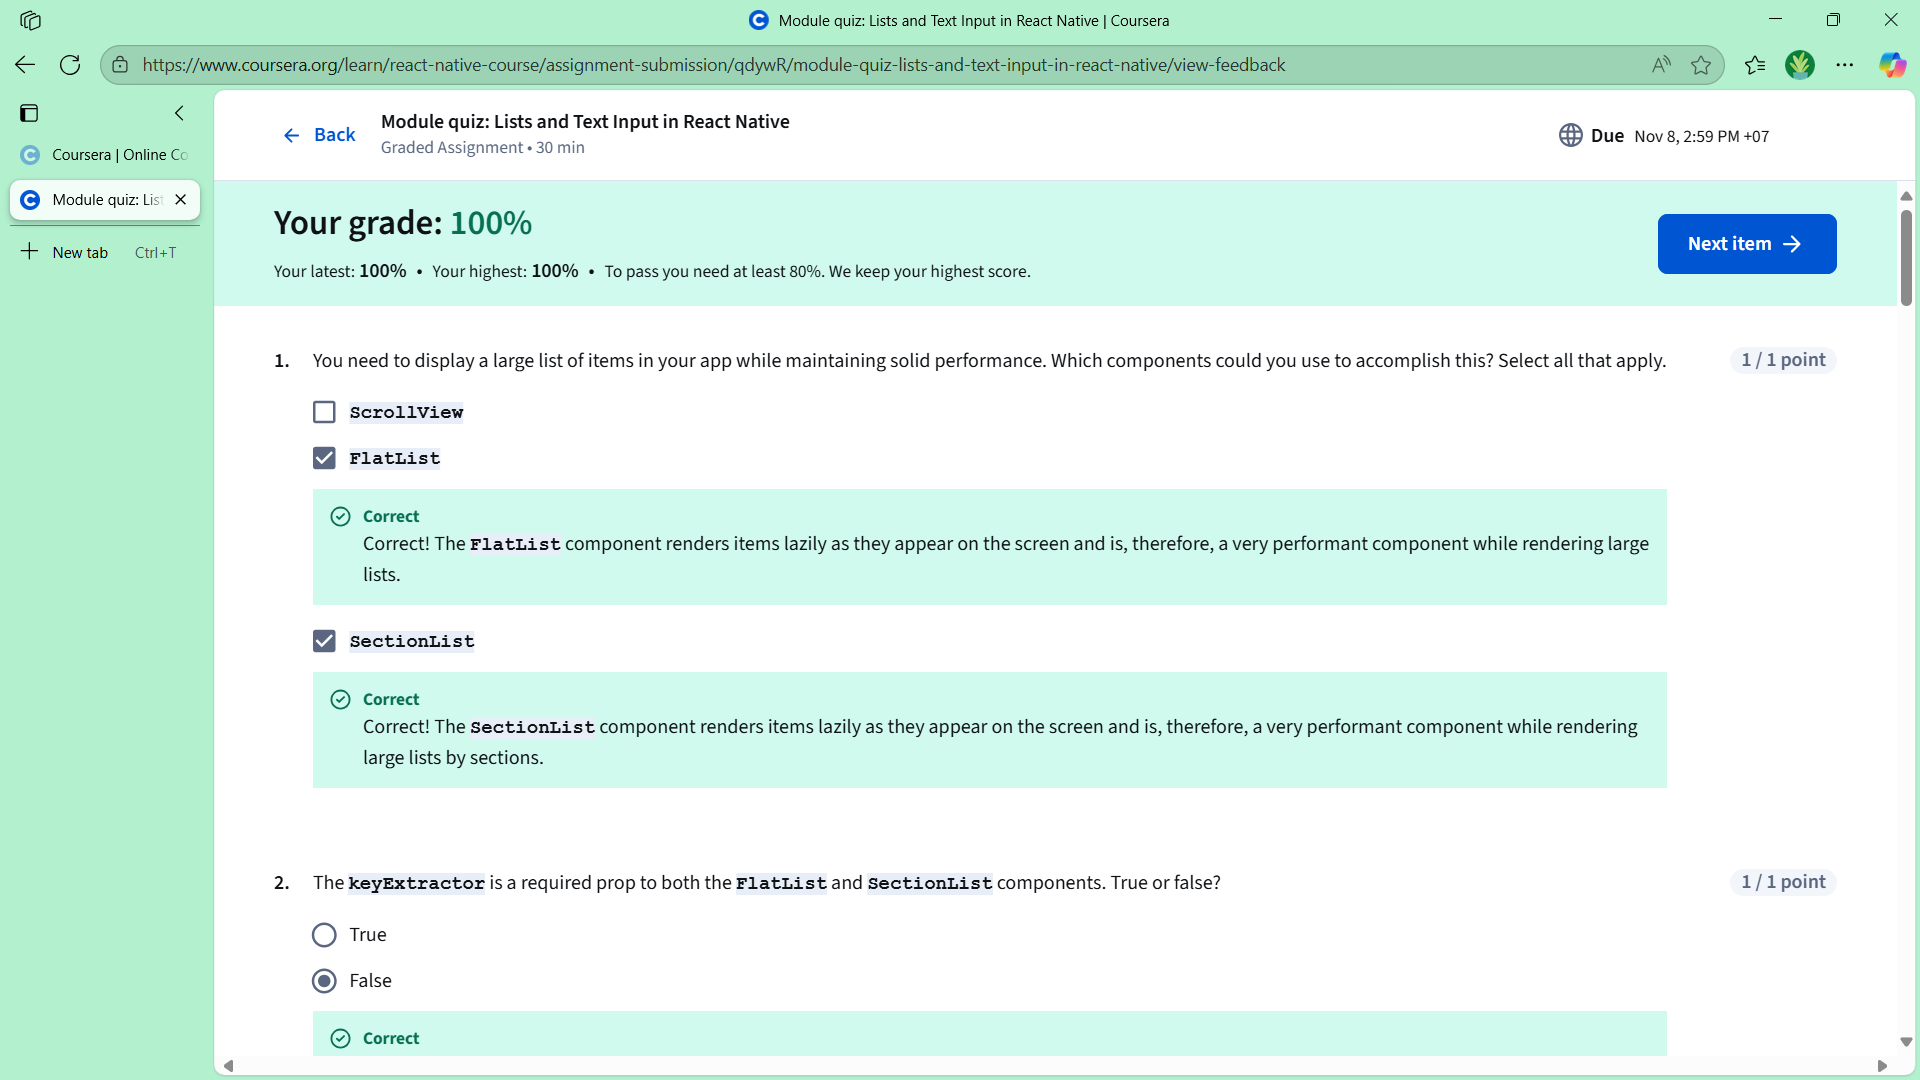
\includegraphics[width=0.5\textwidth]{images/module-quiz.png}
    \caption{Module quiz: Lists and Text Input in React Native}
\end{figure}